\documentclass{beamer}

\usetheme{simple}

\usepackage{scalerel,xparse}
\usepackage{lmodern}
\usepackage[scale=2]{ccicons}
\usepackage{ulem}
\usepackage{tikz}
\usetikzlibrary{positioning,calc,automata}
\usepackage{algorithm}
\usepackage{algorithmic}
\usepackage{caption}
\usepackage{listings}

% Watermark background (simple theme)
\setlength{\parindent}{0cm}
\setwatermark{
\includegraphics[height=8cm]{img/chungus.png}}


\title{CSC363H5 Tutorial 4}
\subtitle{this time in dark theme!}
\date{\today}
\author{Paul ``sushi{\textunderscore}enjoyer'' Zhang}
\institute{University of Chungi}

\NewDocumentCommand\emojisushi{}{
    
\includegraphics{img/1f363.png}
}
\NewDocumentCommand\emojimoyai{}{
    
\includegraphics{img/1f5ff.png}
}

\begin{document}

\maketitle

\begin{frame}{Learning objectives this tutorial}
By the end of this tutorial, you should...
\begin{itemize}
\item Find a totally legal way to obtain the recommended textbook for this course.
\item Read the recommended textbook sections (if you'd like, but I think it's really worth it!).
\item Be able to state the \textit{normal form theorem} and apply it to an example problem.
\item Turn yourself into a moai. \emojimoyai \emojimoyai \emojimoyai
\item Have your internet revoked by your ISP due to piracy.
\item Appreciate the time when I ran tutorials using light theme slides instead of dark theme slides like these.
\end{itemize}
\end{frame}

\begin{frame}{IMPORTANT NOTICE}
sowwy ;-; i had to speedrun those slides, i realized i was covering the wrong content only a few hours prior. i was gonna cover some week 4 material, until i realized people in the friday lecture would probably have no idea what i'm talking about, so i had to quickly remake some slides.

the point of today's tutorial is to introduce you to some proofs that we have skipped in class. 
\end{frame}

\begin{frame}{Readings? What is this, English class?}
Yea, I just discovered that a (recommended) textbook exists for this course! Available for the cheap price of only \$150.
\begin{figure}[placement]
\centering
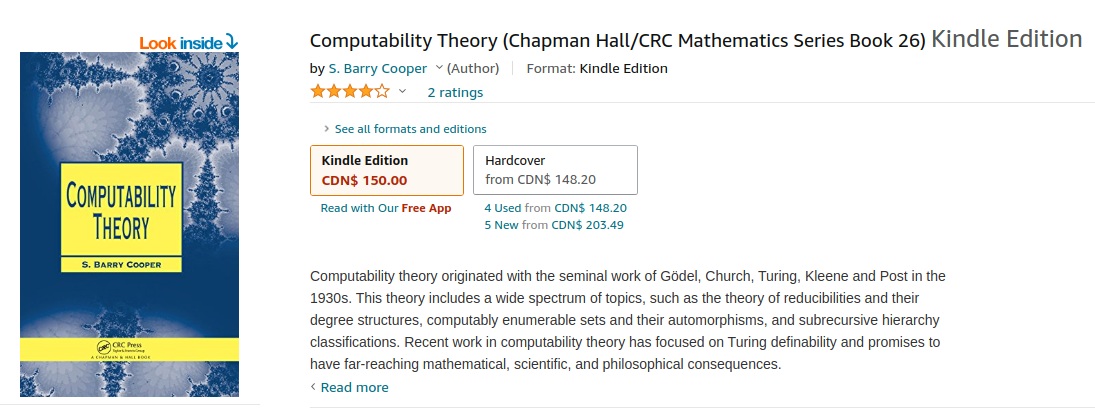
\includegraphics[scale=0.3]{img/book.png}
yea right.
\end{figure}
Trust me, it's worth a read! You will learn cool stuff like \sout{how to solve homework problems} the proof of some theorems skipped in class.

\end{frame}

\begin{frame}{Readings? What is this, English class?}
Just some recommended readings\footnote{not official! just what i think would be useful.} from me to reinforce lecture material:
\begin{itemize}
\item Week 2: sections 2, 4.2, 4.3 (Note the book gives a different definition of Turing machine, but it is equivalent and worth a read!)
\item Week 3: sections 5.1-5.3
\item Week 4: sections 5.2, 10.1 (first page)
\end{itemize}
These recommended readings are certified by \texttt{helo\textunderscore fish.jpg}.
\begin{figure}[h]

\includegraphics[scale=0.3]{img/helo_fish_certified.jpg}
\end{figure}
\end{frame}

\begin{frame}{G*del is back!}
We claimed this statement is true without proving it previously:
\begin{quotation}
Any finite set $A \subseteq \mathbb N$ is computable.
\end{quotation}
Let us prove it.

\vspace{2mm}

\textbf{Task:} Prove the above statement using the Church-Turing Thesis. In other words, describe an algorithm that decides whether some arbitrary $x \in \mathbb N$ is in $A$ or not (within a finite amount of time).\footnote{Note that $A$ is predetermined already: your algorithm does not take $A$ as an input.}

\vspace{2mm}

Hint: If $A$ is finite, we can write $A = \{a_1, a_2, \ldots, a_n\}$.

\vspace{2mm}

\pause

Answer: Given an input $x \in \mathbb N$, do the following:
\begin{align*}
& \text{$i = 1$}\\
& \text{while $i \leq n$:}\\
& \quad \text{if $x = a_i$: return True}\\
& \text{return False}
\end{align*}


\end{frame}


\begin{frame}{Normal Form Theorem!}
\begin{quotation}
We say a set $A \subseteq \mathbb N$ is \textbf{computably enumerable (c.e.)} if $A = \emptyset$ or there exists a computable $f: \mathbb N \to \mathbb N$ such that $A = \text{range}(f)$. 
\end{quotation}

\begin{quotation}
We say a relation $R(\vec{x})$ is in $\Sigma^0_1$ if there exists a computable relation $C(a, \vec{x})$ such that for all $\vec{x}$, $R(\vec{x}) \Leftrightarrow \exists \vec{a} \, C(\vec{a}, \vec{x})$. In other words, when $R$ is thought of as a set,
$$R = \{\vec{x}: \exists \vec{a} \, C(\vec{a}, \vec{x})\}.$$
\end{quotation}

\begin{quotation}
For $e \in \mathbb N$, we denote by $W_e$ the set $\text{dom}(\varphi_e)$, where $\varphi_e$ is the partial recursive function corresponding to the $e$-th Turing machine.
\end{quotation}

\textbf{Task:} Digest those definitions.

\end{frame}


\begin{frame}{Normal Form Theorem!}
Finally, we get to the statement! :D (or D: if you don't like proofs)

\begin{theorem}
Let $A \subseteq \mathbb N$. The following are equivalent:
\begin{enumerate}
\item $A$ is c.e.;
\item $A \in \Sigma^0_1$ (when $A$ is thought of as a unary relation);
\item $A = W_e$ for some $e \in \mathbb N$.
\end{enumerate}
\end{theorem}

We will prove (1) $\Rightarrow$ (2) $\Rightarrow$ (3) $\Rightarrow$ (1). But before we begin, let's try some examples!

\vspace{2mm}

\textbf{Task:} Let $A = \mathbb N$. Show that $A$ is c.e.. Do the same with $A = E$ (the set of even natural numbers).

\pause

Answer: For $A = \mathbb N$, $f(x) = x$ satisfies $\text{range}(f) = A$. For $A = E$, $f(x) = 2x$ satisfies $\text{range}(f) = A$.
\end{frame}

\begin{frame}{Normal Form Theorem!}
\textbf{Task:} Let $A = \mathbb N$. Show that $A \in \Sigma^0_1$ by finding a computable relation $C(a, x)$ such that for all $x \in \mathbb N$, $x \in A$ if and only if there exists $a$ such that $C(a, x)$ holds. In other words,
$$A = \{x \in \mathbb N: \exists a \, C(a, x)\}.$$ 
Do the same with $A = E$ (the set of even natural numbers).

\vspace{2mm}

\pause

Answer: For $A = \mathbb N$, if $C(a, x): a = x$, then
$$A = \{x \in \mathbb N: \exists a \, C(a, x)\}.$$

For $A = E$, if $C(a, x): 2a = x$, then
$$A = \{x \in \mathbb N: \exists a \, C(a, x)\}.$$
\end{frame}

\begin{frame}{Normal Form Theorem!}
\textbf{Task:} Let $A = \mathbb N$. Show that $A = W_e$ for some $e \in \mathbb N$, by finding a Turing machine $P_e$ that halts only on $A$. In other words,
$$A = \{x \in \mathbb N: \text{$P_e$ halts given input $x$}\}.$$
Do the same with $A = E$ (the set of even natural numbers).

\vspace{2mm}

\pause

Answer: For $A = \mathbb N$, let $P_e$ be the Turing machine that halts as soon as it receives any input (so that it halts on all inputs).

For $A = E$, let $P_e$ be the Turing machine that performs the following procedure given input $x$:
\begin{align*}
& \text{if $x \bmod 2 = 0$}:\\
& \quad \text{stop executing!!! D:}\\
& \text{else}:\\
& \quad \text{loop and waste CPU resources.}
\end{align*}
\end{frame}


\begin{frame}{Hope you like proofs.}
Here's the Normal Form Theorem again.
\begin{theorem}
Let $A \subseteq \mathbb N$. The following are equivalent:
\begin{enumerate}
\item $A$ is c.e.;
\item $A \in \Sigma^0_1$ (when $A$ is thought of as a unary relation);
\item $A = W_e$ for some $e \in \mathbb N$.
\end{enumerate}
\end{theorem}

Hopefully with the previous tasks, you have convinced yourself that the Normal Form Theorem holds for computable sets.

\vspace{2mm}
\end{frame}

\begin{frame}{Hope you like proofs.}
(1) $\Rightarrow$ (2): $A$ is c.e. $\Rightarrow$ $A \in \Sigma^0_1$.

\vspace{2mm}

To prove this: suppose $A$ is c.e., so either $A = \emptyset$ or $A = \{f(0), f(1), \ldots\}$. To show $A \in \Sigma^0_1$, we want to write
$$A = \{x \in \mathbb N: \exists a \, C(a, x)\}$$
where $C(a, x)$ is a computable relation.

\vspace{2mm}

\textbf{Task:} Come up with such a computable relation $C(a, x)$ so that $A$ satisfies the above equality. 

\vspace{2mm}

(Hint: I think you will probably need a separate case for $A = \emptyset$).
\end{frame}

\begin{frame}{Hope you like proofs.}
To show $A \in \Sigma^0_1$, we want to write
$$A = \{x \in \mathbb N: \exists a \, C(a, x)\}$$
where $C(a, x)$ is a computable relation.

\vspace{2mm}

\textbf{Task:} Come up with such a computable relation $C(a, x)$ so that $A$ satisfies the above equality. 

\vspace{2mm}

Answer: If $A = \emptyset$, let $C(a, x)$ be the empty relation (false for all $a, x$). Then for any $x \in \mathbb N$, there doesn't exist $a$ such that $C(a, x)$ is true, so
$$\{x \in \mathbb N: \exists a \, C(a, x)\} = \emptyset = A.$$

Otherwise $A = \{f(0), f(1), \ldots\}$ for a computable $f$. Let $C(a, x): f(a) = x$. Since the range of $f$ is $A$, we have
$$\{x \in \mathbb N: \exists a \, C(a, x)\} = \{x \in \mathbb N: \exists a \, f(a) = x\} = A.$$
\end{frame}

\begin{frame}{Hope you like proofs.}
(2) $\Rightarrow$ (3): $A \in \Sigma^0_1 \Rightarrow A = W_e$ for some $e \in \mathbb N$.

\vspace{2mm}

To prove this: suppose $A \in \Sigma^0_1$, so there is a computable relation $C(a, x)$ so that
$$A = \{x \in \mathbb N: \exists a \, C(a, x)\}.$$
To show $A = W_e$ for some $e \in \mathbb N$, we want to produce a Turing machine that only halts on $A$ (since $W_e$ is the set of inputs that make the $e$th Turing machine halt).

\vspace{2mm}

\textbf{Task:} Come up with such a Turing machine (informally describing what it does).
\end{frame}

\begin{frame}{Hope you like proofs.}
\vspace{2mm}
$$A = \{x \in \mathbb N: \exists a \, C(a, x)\}.$$
We want to produce a Turing machine that only halts on $A$.

\vspace{2mm}

\textbf{Task:} Come up with such a Turing machine (informally describing what it does).

\vspace{2mm}

Answer: Let $P_e$ be the Turing machine that does the following given an input $x \in \mathbb N$:
\begin{align*}
& \text{a = 0}\\
& \text{while not $C(a, x)$:}\\
& \quad \text{a += 1}
\end{align*}
This program halts on input $x$ if and only if $x \in A$.
\end{frame}

\begin{frame}{Hope you like proofs.}
(3) $\Rightarrow$ (1): $A = W_e$ for some $e \in \mathbb N$ $\Rightarrow$ $A$ is c.e.

\vspace{2mm}

To prove this: suppose $A = W_e$. If $A = \emptyset$, then $A$ is c.e. by definition and we are done. Otherwise there exists a $p \in A$. We want to find a computable function $f$ such that $A = \text{range}(f)$.

\vspace{2mm}

\textbf{Definition:} We say $\varphi_{e, s}(x) \downarrow$ when $x, e < s$ and the $e$th Turing machine takes $s$ steps or less to halt on $x$.

\textbf{Task:} Digest the above definition.


\vspace{2mm}

\pause

Notice: $x \in W_e$ if and only if $\varphi_{e, s}(x) \downarrow$ for some $s \in \mathbb N$. In other words, $s$ is large enough so that $x, e < s$ and the Turing machine takes $s$ steps or less to halt on $x$.

\textbf{Task:} Argue that we can determine whether $\varphi_{e, s}(x) \downarrow$ or not (in a finite amount of time).


\end{frame}

\begin{frame}{Hope you like proofs.}
(3) $\Rightarrow$ (1): $A = W_e$ for some $e \in \mathbb N$ $\Rightarrow$ $A$ is c.e.

\vspace{2mm}

To prove this: suppose $A = W_e$. If $A = \emptyset$, then $A$ is c.e. by definition and we are done. Otherwise there exists a $p \in A$. We want to find a computable function $f$ such that $A = \text{range}(f)$.

\vspace{2mm}

\textbf{Task:} Show (or convince yourself) that the range of $f$ is exactly $A$, where
$$f(\langle x, s\rangle) = \begin{cases}
x & \varphi_{e, s}(x) \downarrow\\
p & \text{otherwise.}
\end{cases}$$
\end{frame}

\begin{frame}{This finishes the proof!}
\textbf{Task:} Breathe in for 4 seconds, hold your breath for 7 seconds, then slowly release it for 8 seconds. Repeat for 3 minutes. 

\vspace{2mm}

While doing this, imagine you are a 600-year-old giant 50-ton stone on Easter Island in the middle of the Pacific. You have access to a black box that can solve \textit{all} problems in this universe, including non-computable problems such as deciding whether $x \in \mathbb N$ is in the halting set $K$, as it has access to any oracle in existence.

As you breath in and out, you feel your brain expanding. You are filled with \textit{determination}. You can solve any problem. You acknowledge all the suffering and injustice you have received throughout your life, and have ascended beyond any worldly desire. A light breeze brushes up against your coarse stone surface. You feel \textit{at peace}. 

A \textit{Gygis alba} lands on your head. You can hear it chirping amidst the light breeze. You are unbothered, because you have ascended beyond life.

You are a Moai. \emojimoyai\emojimoyai\emojimoyai


\end{frame}

\begin{frame}{\emojimoyai\emojimoyai\emojimoyai\emojimoyai\emojimoyai\emojimoyai}

\begin{figure}[h]
\centering

\includegraphics{img/moai.jpg}
\end{figure}


\end{frame}

\begin{frame}{\emojimoyai\emojimoyai\emojimoyai\emojimoyai\emojimoyai\emojimoyai}
Now that you have attained knowledge of this universe, you may prove the following:
\begin{quotation}
Let $A \subseteq \mathbb N$. $A$ is c.e. if and only if there exists a partial computable function $f$ such that $A = \text{range}(f)$.
\end{quotation}

\textbf{Task:} Prove the above using the normal form theorem (written below).

\begin{theorem}
Let $A \subseteq \mathbb N$. The following are equivalent:
\begin{enumerate}
\item $A$ is c.e.;
\item $A \in \Sigma^0_1$ (when $A$ is thought of as a unary relation);
\item $A = W_e$ for some $e \in \mathbb N$.
\end{enumerate}
\end{theorem}


Hint: For proving the $\Leftarrow$ direction (which is more difficult), show $A$ satisfies condition 2 in the above theorem. You may want to use $\varphi_{e, s}(x) \downarrow$ somewhere in this direction.


\end{frame}

\begin{frame}{\emojimoyai\emojimoyai\emojimoyai\emojimoyai\emojimoyai\emojimoyai}
Now that you have attained knowledge of this universe, you may prove the following:
\begin{quotation}
Let $A \subseteq \mathbb N$. $A$ is c.e. if and only if there exists a partial computable function $f$ such that $A = \text{range}(f)$.
\end{quotation}

Proof: ($\Rightarrow$) Suppose $A$ is c.e.. Then either $A = \emptyset$ or $A = \text{range}(f)$ for some \textit{computable} function $f$. If $A = \emptyset$, then $A$ is the range of the empty partial computable function (always undefined). Otherwise $A = \text{range}(f)$ (and $f$ is partial computable since it is computable).

\vspace{2mm}

($\Leftarrow$) Let $A = \text{range}(f)$ for some partial computable $f$. Then $f = \varphi_e$ for some $e \in \mathbb N$ (since $f$ can be emulated by a Turing machine). Define the relation
$$C(s, x, y): \varphi_{e, s}(x) \downarrow = y.$$
Then 
$$A = \{y \in \mathbb N: \exists (s, x)  \, C(s, x, y) \}.$$


(Formally I should have used $C(\langle s, x \rangle, y)$ for the relation.)
\end{frame}

\begin{frame}{Thanks for watching my video. For more information, please visit \texttt{sjorv.github.io} for a giveaway of two \$GME shares.}

\begin{columns}
\column{0.4\linewidth}
If you'd like to cheat on the homework, please stay for office hours! :D
\vspace{4mm}

If not, then bye. ;-; 

To help you on your homework, please try the following proof methods.
\column{0.5\linewidth}
\begin{figure}[h]
\centering
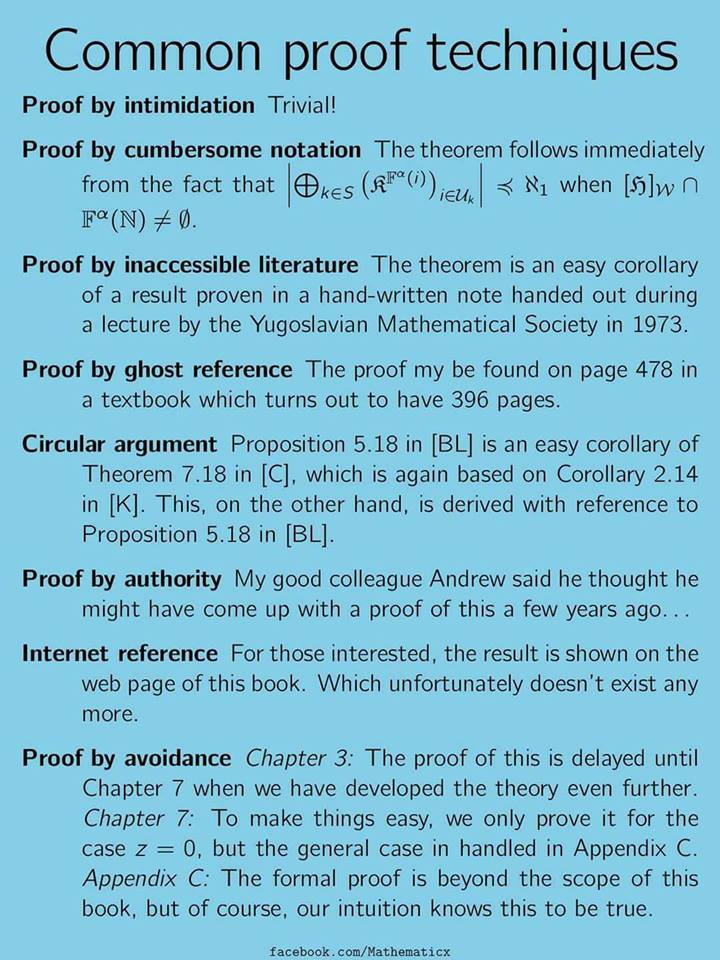
\includegraphics[scale=0.21]{img/proof_techniques.png}
\end{figure}
\end{columns}


\end{frame}










\end{document}